\documentclass[12pt,a4paper,final]{article}
\usepackage[latin1]{inputenc}
\usepackage[authoryear]{natbib}
\usepackage[T1]{fontenc}
\usepackage{amsmath}
\usepackage{amsfonts}
\usepackage{amssymb}
\usepackage{setspace}
\usepackage[pagewise]{lineno}
\usepackage{graphicx,epstopdf}
\usepackage{subfigure}
\usepackage[verbose,a4paper,tmargin=2.4cm,bmargin=2.4cm,lmargin=2.4cm,rmargin=2.4cm]{geometry}
\usepackage{setspace}
%\doublespacing

% Use the PLoS provided bibtex style
\bibliographystyle{plos2009}

\usepackage{color,ulem} % package for text color comments

\author{Vasilis Dakos and Leo Lahti}

\title{
\begin{figure}[h]
\begin{left}

\includegraphics[scale=0.8]{logoEWS.eps}
\end{left}
\end{figure}
\\
Early Warning Signals Toolbox: 
\\ A novel approach for Detecting Critical Transitions
}

\begin{document}
\maketitle

\section{In an nutshell} %Overview
Critical transitions have been identified in seemingly disparate systems ranging from ecology and climate to medicine and finance (Scheffer et al. 2001; Scheffer 2009). %Global finance occasionally suffers from market crashes (May et al. 2008), while asthma attacks (Venegas et al. 2005) and epileptic seizures (McSharry et al. 2003) are examples of sudden medical systemic failures. Abrupt shifts in ocean circulation have occurred in the past climate (Rahmstorf 2002) and may be triggered again under present trends of global environmental conditions (Lenton et al. 2008).
Acknowledging the existence of such critical transitions is only the first step for avoiding them. What we are currently lacking are tools that we can use to foresee such upcoming transitions. Being able to quantify the probability of a critical transition happening would be of unperceived value. Unfortunately, for most systems, we neither have enough records of past transitions nor reliable models to study their behavior. Nonetheless, recent work has proposed an alternative, novel way of approaching this challenge. What if, instead of building case-specific models or indicators, we could be able to measure the resilience of a system- and thus its proximity to a critical transition- using a more generic approach? Complex systems theory appears to have provided us with a potential solution: \textit{\textbf{generic early-warning signals}} for critical transitions (Scheffer et al. 2009). 
\\
\\
Here, we present our newly developed \textbf{Early Warning Signal Toolbox} designed for the \textbf{estimation} and \textbf{visualization} of fingerprints of upcoming critical transitions from time series data. Our toolbox is characterized by three unique features. \textit{\textbf{First}}, it is of truly generic nature which means that it can be used for any type of system that may experience a critical transition. \textit{\textbf{Second}}, it is based on highly sophisticated published methods that have been already tested in real world cases. \textit{\textbf{Third}}, it is easy to use and it is developed under a  open-access, widely-used, statistical program (R Project for Statistical Computing\footnote{http://www.r-project.org}). In what follows we explain in laymen terms the theory behind the development of our toolbox, we present how the toolbox works by providing an example, and we explain how this toolbox can have broader benefits for the understanding and management of complex systems in the future.  

\section{The Early Warning Signals Toolbox - Theory} 

\subsection{Why should we expect Early Warnings before Critical Transitions?}
A simple way to understand why we should expect early warnings before critical transitions is to think of the behavior of a system as the motion of a ball in a landscape of valleys and hilltops (Fig. 1 a). Balls represent the state of the system. Valleys correspond to the basins of attraction of alternative stable states of the system. The width and the steepness of the basin of attraction determine the capacity of the system to absorb a perturbation without shifting to an alternative state, and reflects the resilience of the state of the system. As conditions bring the system close to a critical transition (Fig. 1b), the basin of attraction of the current state of the system shrinks and so does its resilience: even a tiny perturbation is enough to shift the sphere to the alternative valley. At the same time, the steepness of the basin of attraction becomes lower: this means that the same perturbation that may not tip the system, it will definitely take longer to dissipate due to the phenomenon of \textit{\textbf{critical slowing down}} (Fig. 1 b). \textit{Mathematically}, critical slowing down is connected to the fact that close to the critical transition the dominant eigenvalue of the system at equilibrium vanishes and has been proven to be be universal prior to critical transitions  (Wissel 1984; Strogatz 1994). \textit{Practically}, critical slowing down enables us to probe the dynamics of the system in order to assess its resilience and the risk of an upcoming transition. The long time required by a system to recover from a perturbation can serve as early-warning signal for an approaching tipping point (van Nes & Scheffer 2007) (Fig. 1 a1, b1).

\begin{figure}[h]
\begin{center}
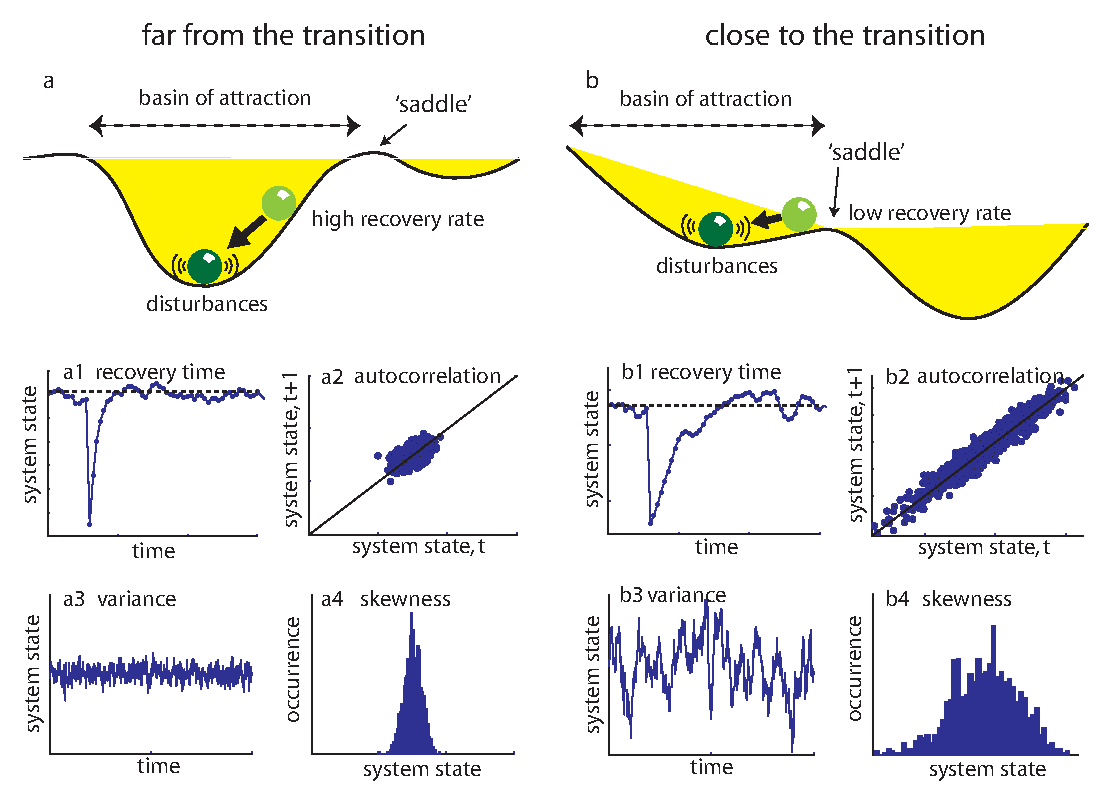
\includegraphics[scale=0.8]{figure1.eps}
\caption{Early-warnings in the dynamics of a system as it approaches a critical transition. Far from the transition resilience is high (a): the system lies in a broad and steep basin of attraction. Small disturbances are damped by high recovery rates back to equilibrium. As a result the time to recover from perturbations is short (a1), the dynamics are characterized by low correlation between subsequent states (a2), low variance (a3), and low skewness (a4). Close to transition resilience is low (b): the system lies in a narrow and flat basin of attraction. Small disturbances are not effectively damped due to critical slowing down. As a result the time to recover from perturbations is short (b1), the dynamics are characterized by high correlation (b2), high variance (b3), and high skewness (b4).}
\end{center}
\label{fig:ews_theory}
\end{figure}

\subsection{What are Early Warning Signals?}
While an increase in recovery time after a disturbance is the most direct indicator of the vicinity to a tipping point, for most natural systems it will be very difficult to measure it systematically. Take for instance the impossibility of conducting a perturbation experiment for measuring the resilience of the thermohaline circulation. The fact, however, that all systems are permanently subjected to natural perturbations allows us to identify an approaching tipping point indirectly. First, slowing down leads to an \textit{\textbf{increase in autocorrelation}} (Ives 1995; Held & Kleinen 2004): the state of the system resembles its previous state when it is close to a tipping point (Fig. 1 a2, b2). The resulting increase in `memory' of the system can be measured in the frequency spectrum of the system by simply looking at lag-1 autocorrelation in the pattern of fluctuations (Held & Kleinen 2004). Second, there is an \textit{\textbf{increase in variance}} (Van Nes & Scheffer 2003; Carpenter & Brock 2006) prior to a tipping point: the state of the system will fluctuate more widely around its equilibrium. As perturbations accumulate and are not damped fast enough due to critical slowing down, the variance in the state of the system increases (Fig. 1 a3, b3). Also, the basin of attraction usually, but not necessarily, becomes asymmetric close to a transition (Scheffer et al. 2009) (Fig. 1 a, b). Such asymmetry causes the state of the system to spend more time in the flatter part of the attraction basin. As a result there is an \textit{\textbf{increase in skewness}} (Guttal & Jayaprakash 2008) in the distribution of the monitored system state before a transition (Fig. 1 a4, b4).

\section{The Early Warning Signals Toolbox - Application}
\subsection{General characteristics}
The Early Warning Signals Toolbox is designed to \textbf{estimate} and \textbf{visualize} a series of \textbf{14 different indicators} that reflect the above-described distinct changes in the signal properties of a system prior to a critical transition (Table 1). In particular:
\begin{itemize}
\item The toolbox works with time series collected by monitoring the state of a system that we suspect it might undergo a critical transition. It requires no more information to a practitioner other than the time series derived from the system.
\item There is no restriction in the type of data that can be processed. Time series may be temperature data, nutrient concentrations, brain activity, stock marker indices or similar. 
\item The versatility of the toolbox allows to study both real world data as well as simulated time series derived from models that are, for instance, developed to understand climatic transitions, ecological shifts or social collapses.
\end{itemize}


\begin{table}[h]
\centering
\caption{List of methods and indicators estimated by the Early Warning Signals Toolbox}  \\ [1ex]
\begin{tabular}{l l}% c c }
\hline
\hline
%\textbf{Method/ Indicator}\\%	&	Rising memory	&	Rising variability	&	Flickering	\\ [0.5ex]
%\hline
Autocorrelation at-lag-1 &	%&	x	&		&	\\
Autoregressive coefficient of AR(1) model	\\ %&	x	&		& 	\\
Return rate &	%&	x	&		&	\\
Spectral density \\%	&	x	&		&	\\
Spectral ratio &	%&	x	&		&	\\
Spectral exponent\\	%&	x	&		&	\\
Standard deviation &	%&		&	x	&	x	\\
Coefficient of variation\\	%&		&	x	&	x \\
Skewness &	%&		&	x	&	x \\
Kurtosis	\\%&		&	x	&	x \\
Conditional heteroskedasticity	&%&		&	x	&	x	\\
BDS test	\\%&		&	x	&	x	\\
Nonparametric drift-diffusion-jump models	&%&	x	&	x	&	x	\\
Potential analysis	\\ [0.5ex]%&		&		&	x	\\ [1ex]
\hline
\hline
\end{tabular}
\label{methods_table}
\end{table}%

\subsection{An example}
We are not going here to present the full capacity of our toolbox. Instead, we are going to focus only on a subset of flagship indicators that are the most promising for the detection of critical transitions. For this, the toolbox provides a \textbf{Quick Detection Analysis (QDA)} that we are going to demonstrate in detail.
   
   
   data sources
   time series - here examples
   
\textcolor{blue}{(short video that only goes with the example?)}
   
\subsection{Resources} 
   
   (webpage, CRAN package, github)
   sp�cifications (RShiny background,,,)
   
   5. there is a whole support material (webpage, tutorials, methodological papers)
   
\section{Potential impact and future perspectives}
One of the most distinct features of our proposed toolbox is its dynamic character and complimentary functionality.

1. it can be used for online as well as after 
2. it can be part of any other tool
3. can work with simulated data and real data.
4. can be further developed- keeping up pace with on going research. This is reflected by our choice to develop this tool in the R statistical computing environment and to make it available on open source project development platforms like github. is related to the fact that we 
\textcolor{blue}{(@Leo: some on open source computing and R?)}


\end{document}

